\documentclass[aspectratio=169]{beamer}
%\documentclass[aspectratio=43]{beamer}
%\documentclass[newPxFont,sthlmFooter]{beamer}
\usetheme{sthlm}
%\usecolortheme{sthlmv42}

%-=-=-=-=-=-=-=-=-=-=-=-=-=-=-=-=-=-=-=-=-=-=-=-=
%        LOADING PACKAGES
%-=-=-=-=-=-=-=-=-=-=-=-=-=-=-=-=-=-=-=-=-=-=-=-=
\usepackage[utf8]{inputenc}
\usepackage{lscape}
\usepackage{tikz}
\usepackage{marvosym}
\usepackage{chronology}
\usepackage[english]{babel}
\definecolor{airforceblue}{rgb}{0.2,0.2,0.7}
\usepackage{xcolor}
\usepackage{float}
%\spanishdecimal{.}
\renewcommand{\event}[3][e]{%
  \pgfmathsetlength\xstop{(#2-\theyearstart)*\unit}%
  \ifx #1e%
    \draw[fill=black,draw=none,opacity=0.5]%
      (\xstop, 0) circle (.2\unit)%
      node[opacity=1,rotate=45,right=.2\unit] {#3};%
  \else%
    \pgfmathsetlength\xstart{(#1-\theyearstart)*\unit}%
    \draw[fill=black,draw=none,opacity=0.5,rounded corners=.1\unit]%
      (\xstart,-.1\unit) rectangle%
      node[opacity=1,rotate=45,right=.2\unit] {#3} (\xstop,.1\unit);%
  \fi}%

%Dirección de la imágenes
\graphicspath{ {images/} }



\newtheorem{teo}[theorem]{Teorema}
\newtheorem{definicion}[theorem]{Definici\'on}
\newtheorem{lema}[theorem]{Lema}
\newtheorem{coro}[theorem]{Corolario}
\newtheorem{propo}[theorem]{Proposici\'on}
\newtheorem{remarks}[theorem]{Notas}
\newtheorem{remark}[theorem]{Nota}
\newtheorem{claim}[theorem]{Afirmaci\'on}
%\newtheorem{examples}[theorem]{Ejemplos}
%\newtheorem{algorithm}{Algoritmo}[section]
\newtheorem{eje}[theorem]{Ejemplo}
\newtheorem{conjeture}[theorem]{Conjetura}
\newtheorem{question}[theorem]{Pregunta}
\usepackage{ulem}


\DeclareFontFamily{U}{mathx}{}
\DeclareFontShape{U}{mathx}{m}{n}{<-> mathx10}{}
\DeclareSymbolFont{mathx}{U}{mathx}{m}{n}
\DeclareMathAccent{\widehat}{0}{mathx}{"70}
\DeclareMathAccent{\widecheck}{0}{mathx}{"71}
\renewcommand{\check}{\widecheck}

%-=-=-=-=-=-=-=-=-=-=-=-=-=-=-=-=-=-=-=-=-=-=-=-=
%        BEAMER OPTIONS
%-=-=-=-=-=-=-=-=-=-=-=-=-=-=-=-=-=-=-=-=-=-=-=-=

%\setbeameroption{show notes}

%-=-=-=-=-=-=-=-=-=-=-=-=-=-=-=-=-=-=-=-=-=-=-=-=
%
%	PRESENTATION INFORMATION
%
%-=-=-=-=-=-=-=-=-=-=-=-=-=-=-=-=-=-=-=-=-=-=-=-=

\title[]{\Large\centering
\color{airforceblue}Modelo predictivo de la producción de aguacates en Michoacán: desde la siembra hasta la cosecha}
%\\


\author{{\small \textsc{presenta}}\centering{\\Isaac Vázquez Mendoza \\ {\small\textsc{
		bajo la dirección de}}\\ Dra. Magali Arellano Vázquez}}


\institute{}

\begin{document}
	\begin{frame}[noframenumbering]
		%\begin{center}
		%	\includegraphics[scale=0.5]{Encabezado.png}
		%\end{center}
		
		\begin{minipage}{0.15\textwidth}
			\centering
			\hspace{0.3cm}\vspace{-0.6cm}
\includegraphics[scale=0.23]{images/INFOTEC.jpg}
		\end{minipage}%
		\begin{minipage}{0.65\textwidth}
			\centering \vspace{0.5cm}
			\hspace{1cm}INFOTEC
			
			\hspace{1cm}Centro de Investigación e Innovación en TIC
                \hspace{1cm}
   
		\end{minipage}%
		\begin{minipage}{0.2\textwidth}
			
\includegraphics[width=.5cm]{tr.png}
                \hspace*{0.5cm}%
\includegraphics[scale=0.08]{images/EncuentroGarza.png}
		\end{minipage}
		\date{}
		\titlepage
		
		
		
	\end{frame}
%-=-=-=-=-=-=-=-=-=-=-=-=-=-=-=-=-=-=-=-=-=-=-=-=
%
%	TITLE PAGE
%
%-=-=-=-=-=-=-=-=-=-=-=-=-=-=-=-=-=-=-=-=-=-=-=-=

%\begin{frame}[plain]
%	\titlepage
%\end{frame}

%-=-=-=-=-=-=-=-=-=-=-=-=-=-=-=-=-=-=-=-=-=-=-=-=
%
%	TABLE OF CONTENTS: OVERVIEW
%
%-=-=-=-=-=-=-=-=-=-=-=-=-=-=-=-=-=-=-=-=-=-=-=-=

%\begin{frame}{Index}
%	\tableofcontents
%\end{frame}

\definecolor{mygray}{gray}{0.95}

{
	\setbeamercolor{background canvas}{bg=mygray}
	\begin{frame}{Mapa de contenidos}
		\begin{itemize}
			\color{airforceblue}
			\item Motivación del problema
		\end{itemize}
	\end{frame}
}

\begin{frame}{Motivación del problema}
	\vspace{-1.5cm} \centering
	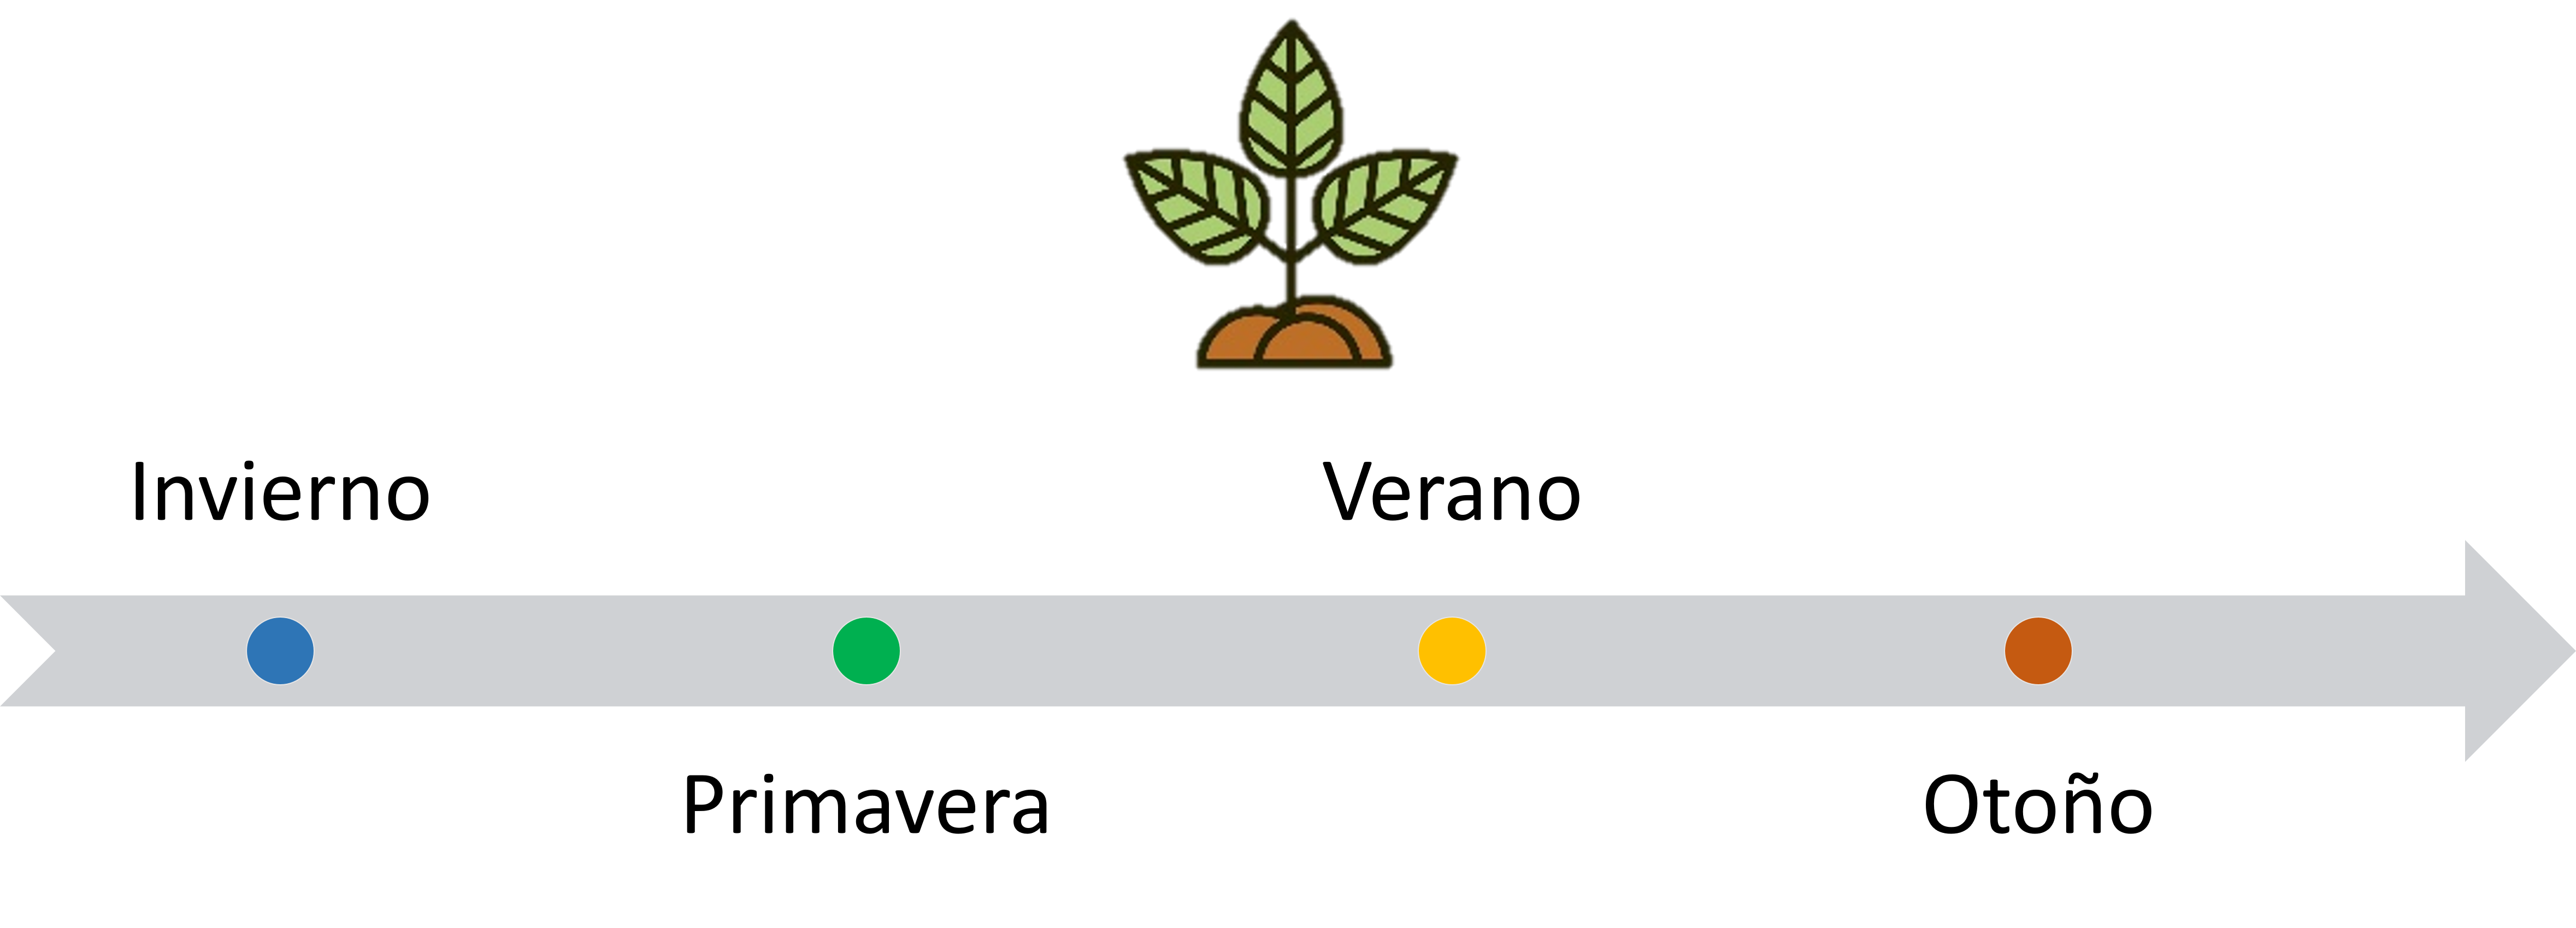
\includegraphics[width=\textwidth]{images/Choice.png}
\end{frame}

\begin{frame}{Motivación del problema}
	\vspace{-1cm}\centering
	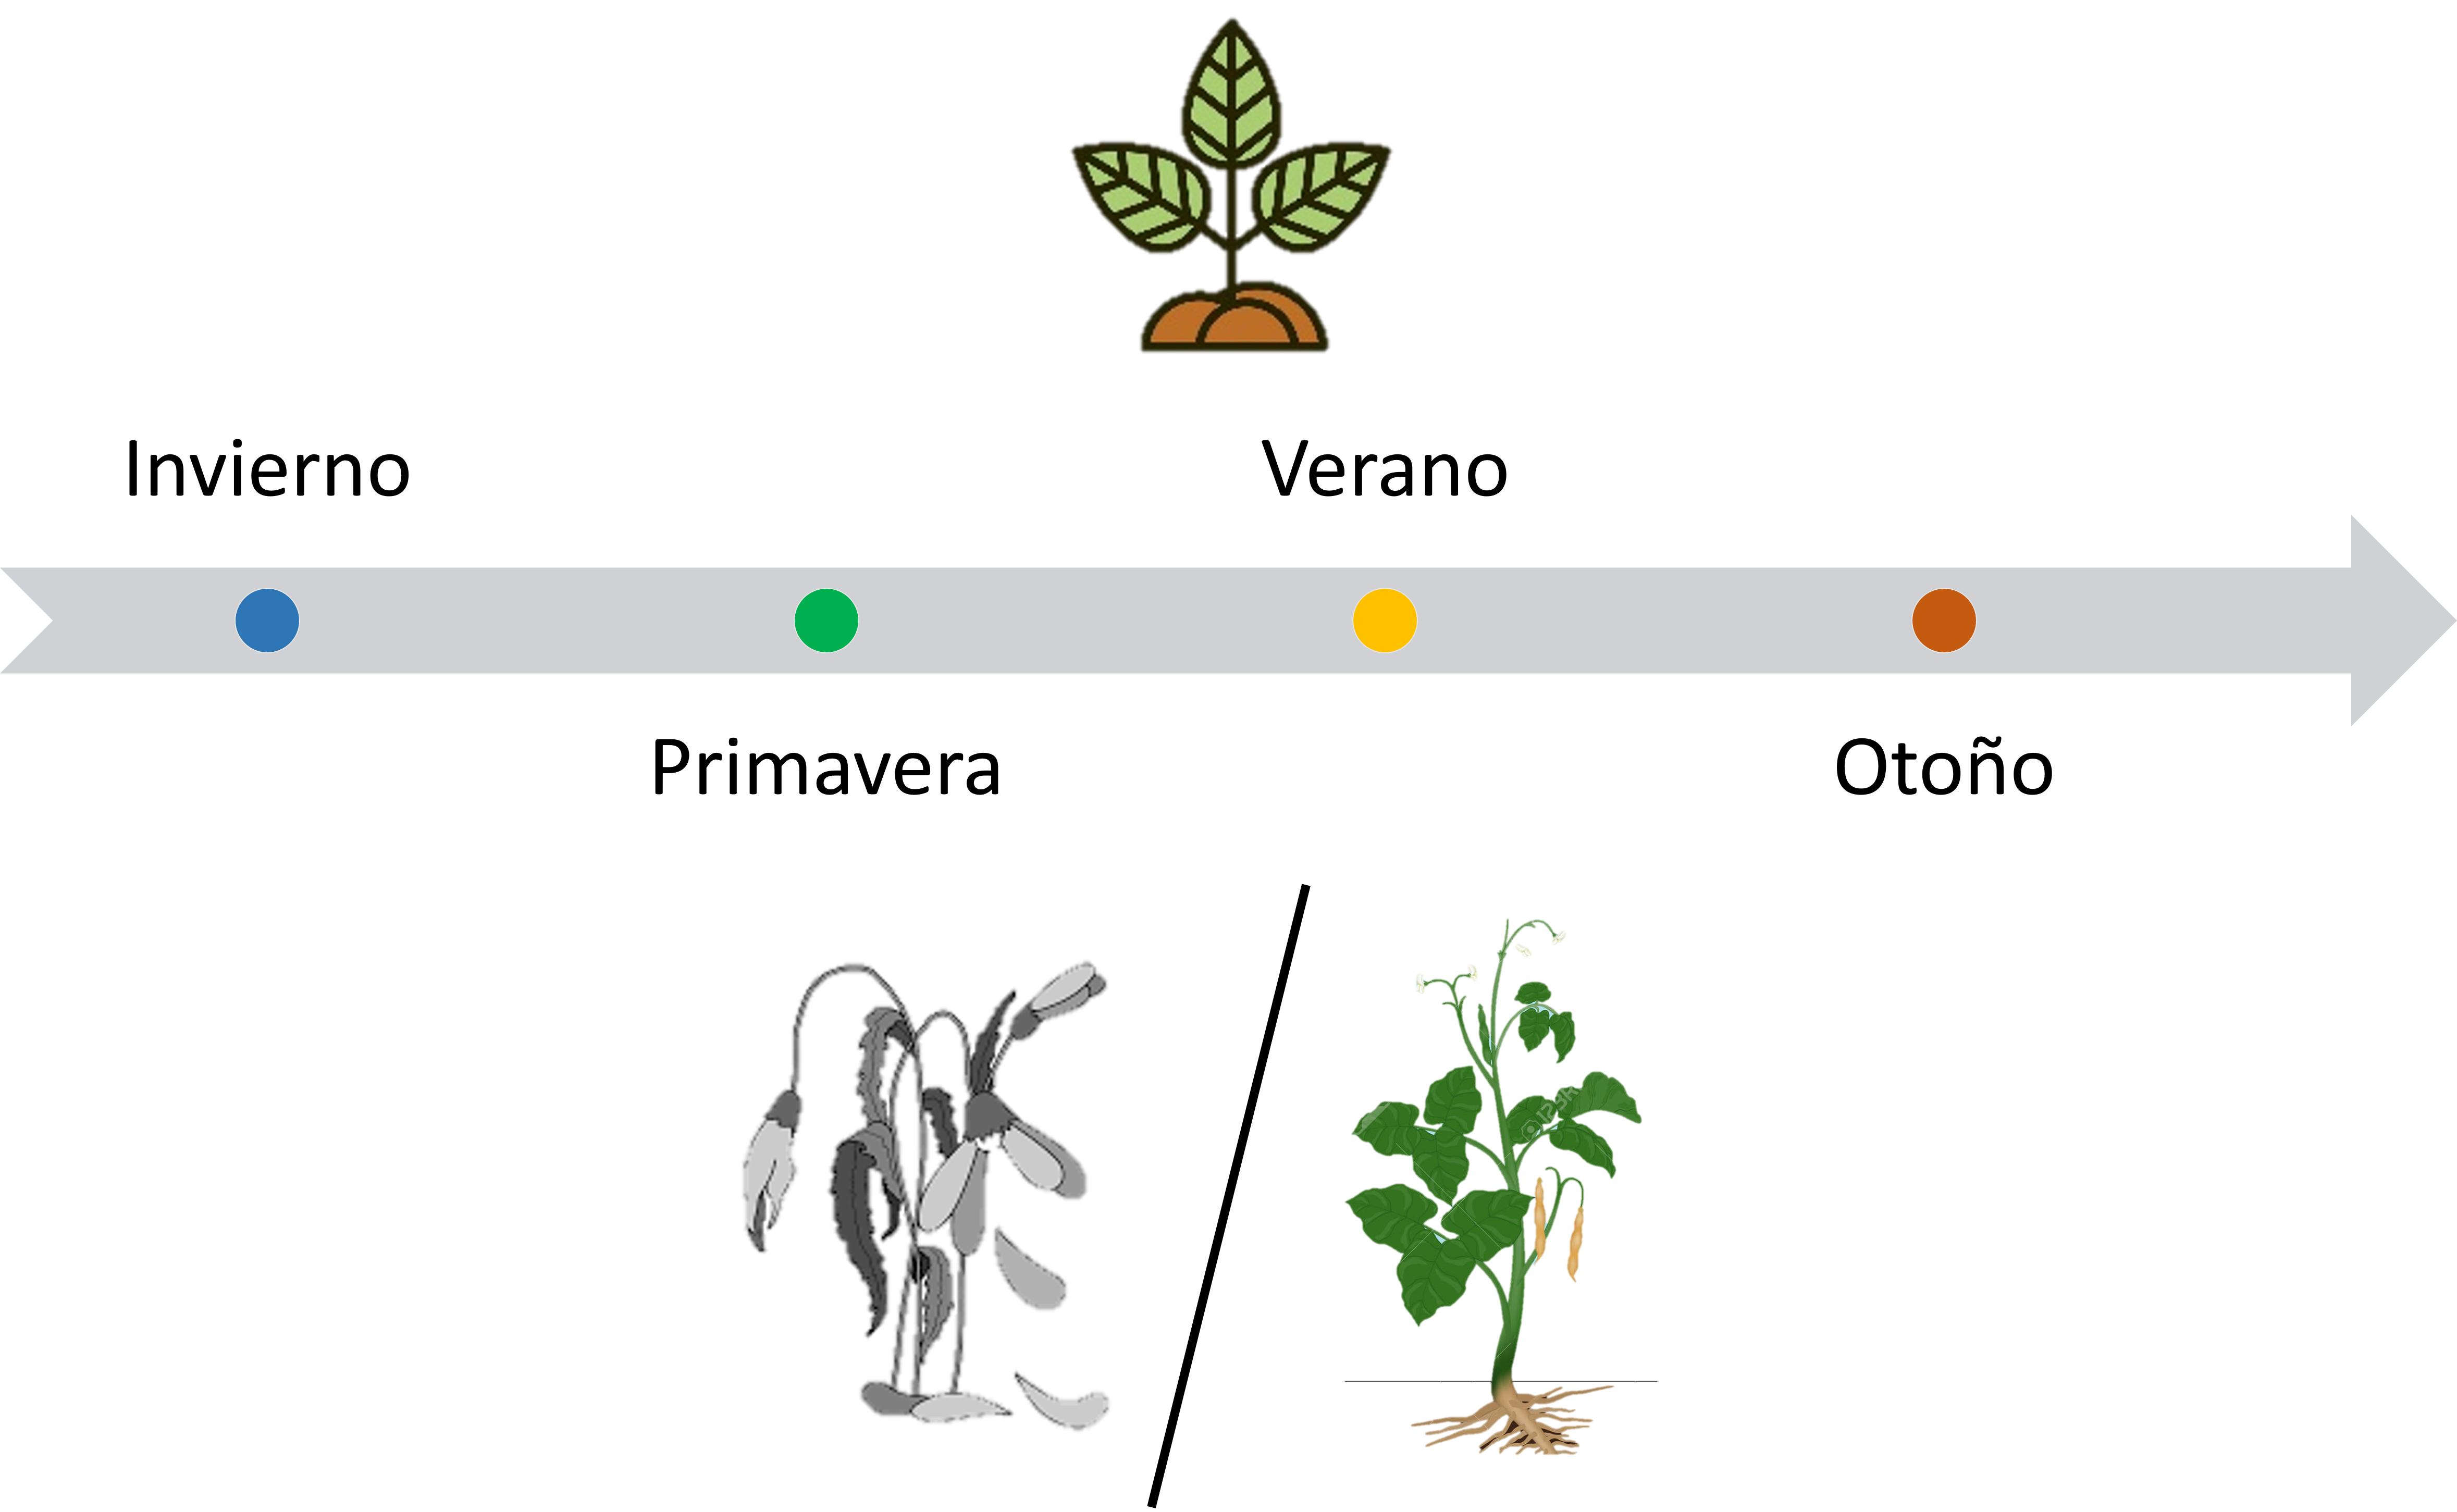
\includegraphics[width=0.9\textwidth]{images/Survival.png}
\end{frame}

\begin{frame}{Motivación del problema}
	 \vspace{-1cm}
	 \centering
	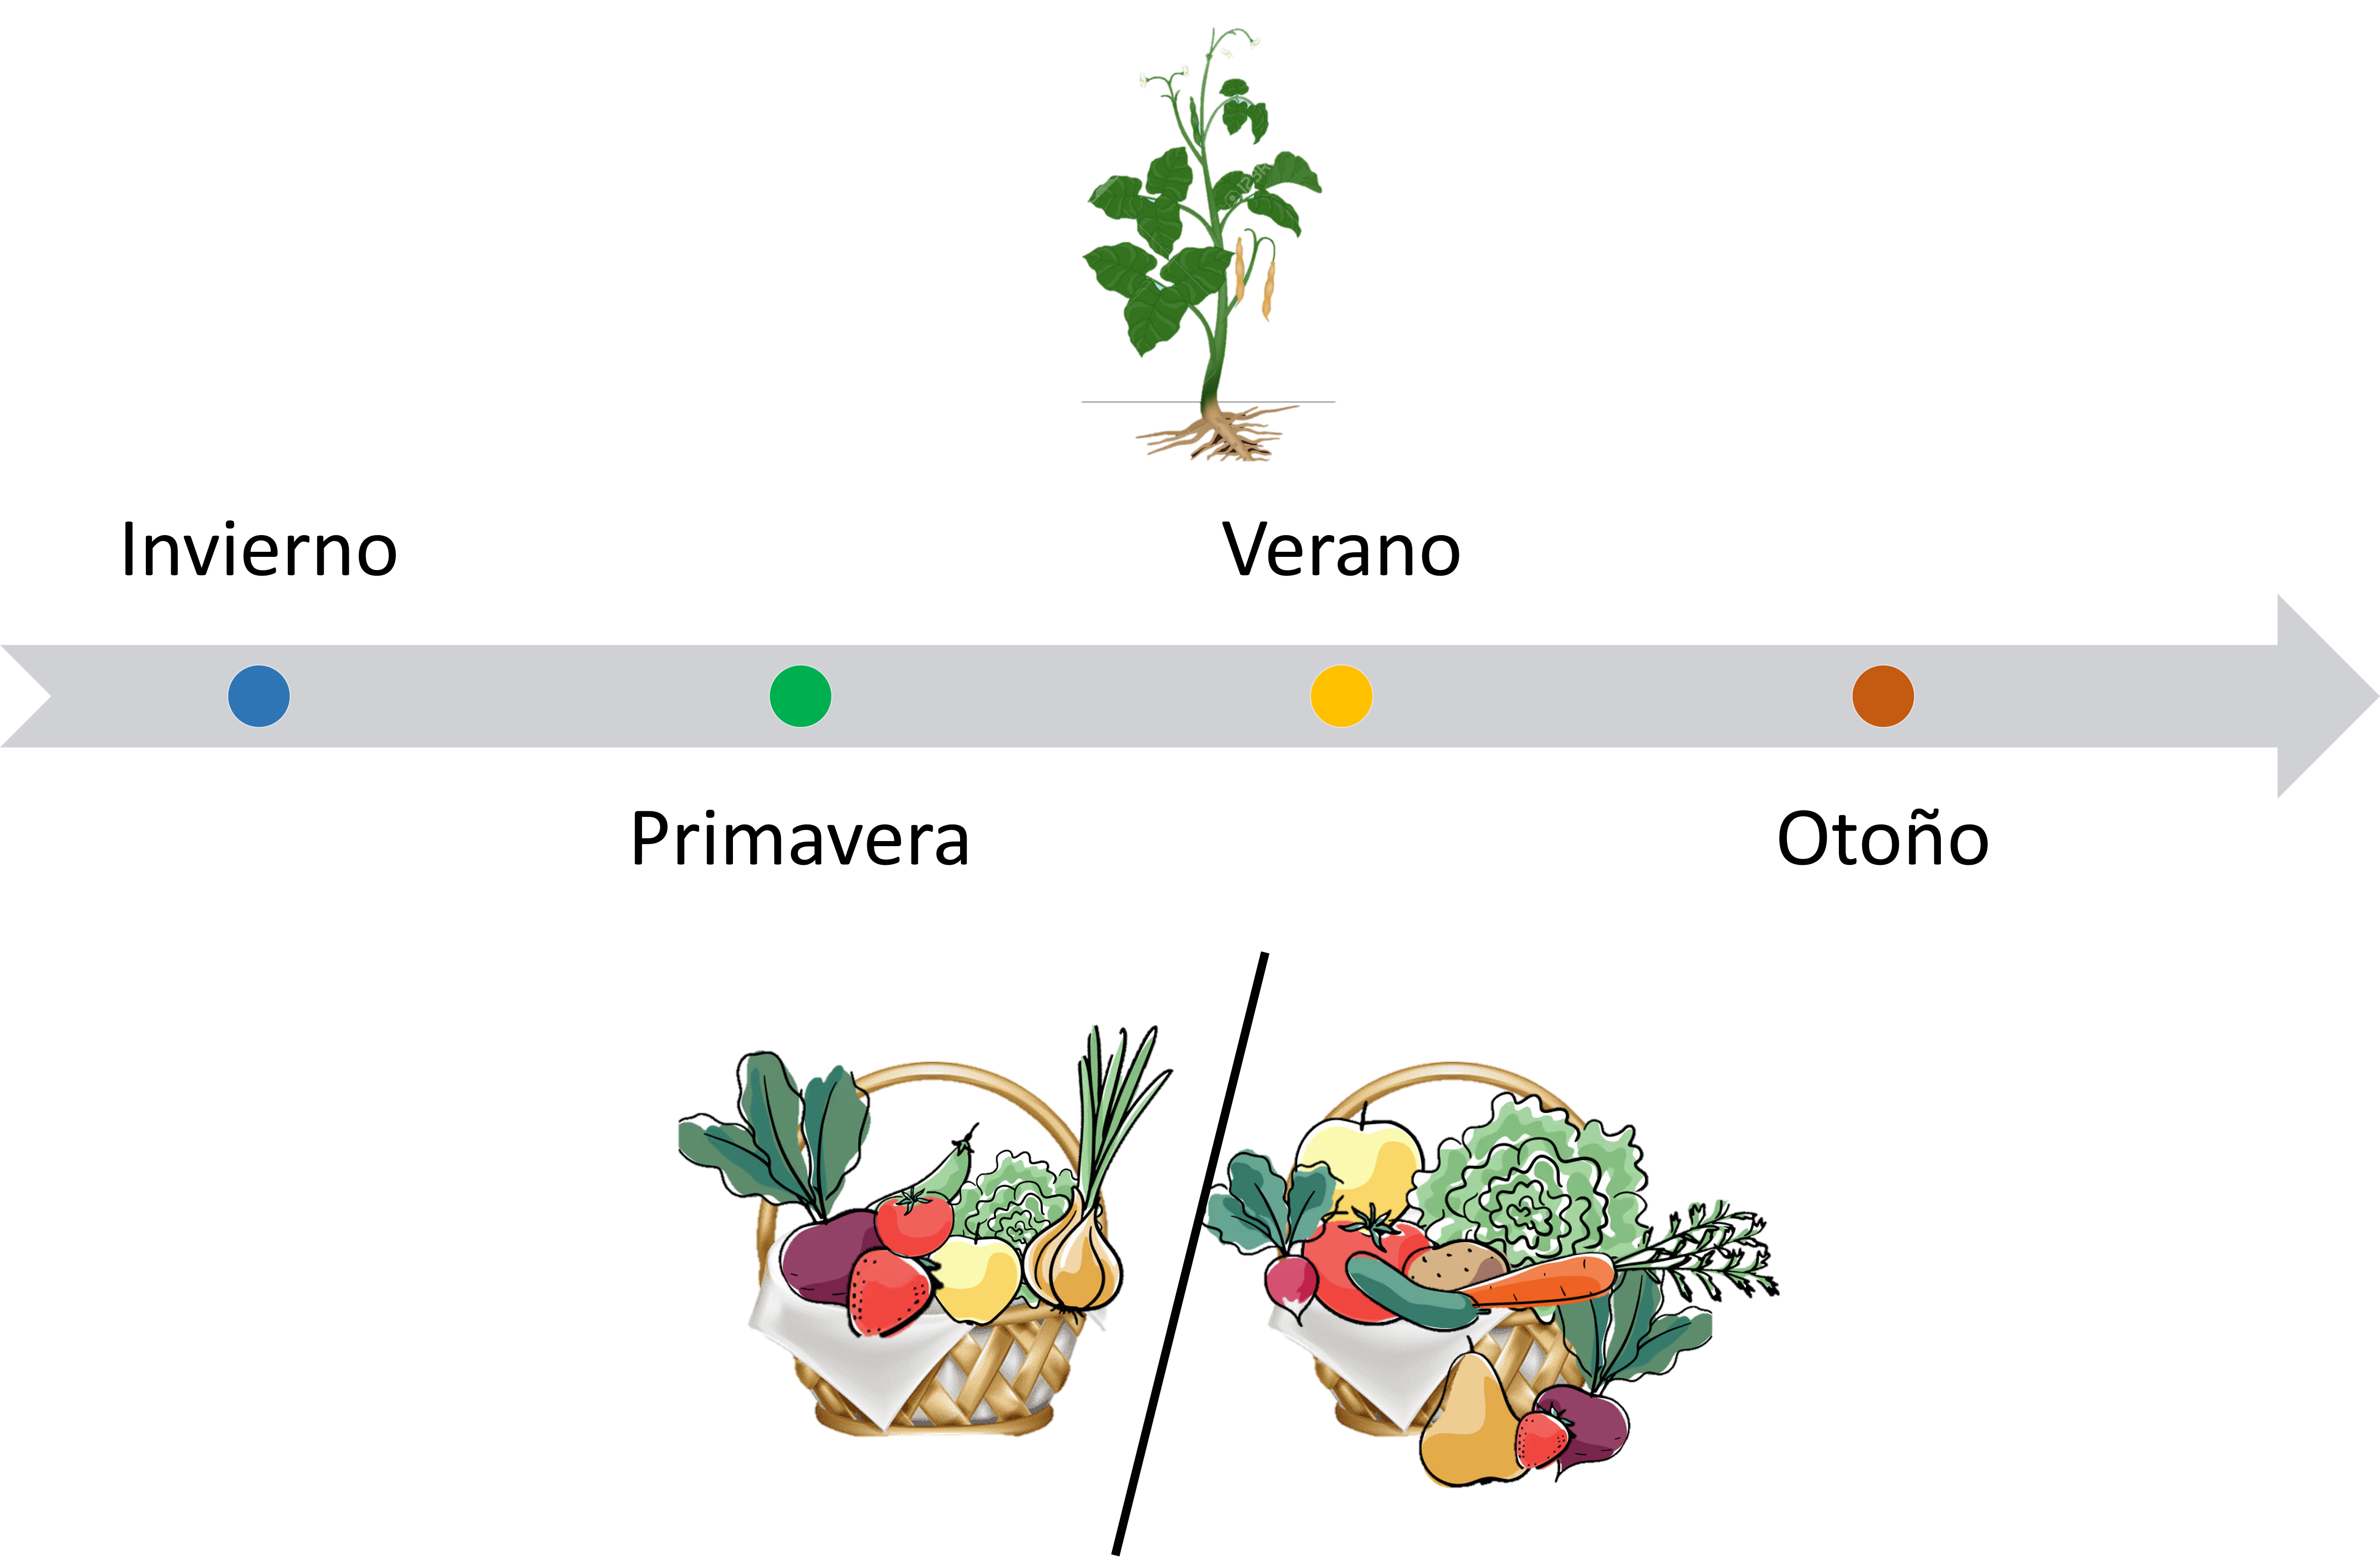
\includegraphics[width=0.9\textwidth]{images/Production.png}
\end{frame}


\begin{frame}{Motivación del problema}
\begin{block}{\centering Proceso de decisión}
	\begin{minipage}{0.5\textwidth}
		\pause\begin{itemize}
			\item Conocimiento ancentral.
			\item Sistematización y mecanización.
			\item Estudios científicos.
			\item Interacciones multidisciplinarias.
		\end{itemize}
	\end{minipage}%
	\begin{minipage}{0.5\textwidth}
			 \phantom{text}
			\phantom{text}
			\phantom{text}
			\phantom{text}
	\end{minipage}
\end{block}
\centering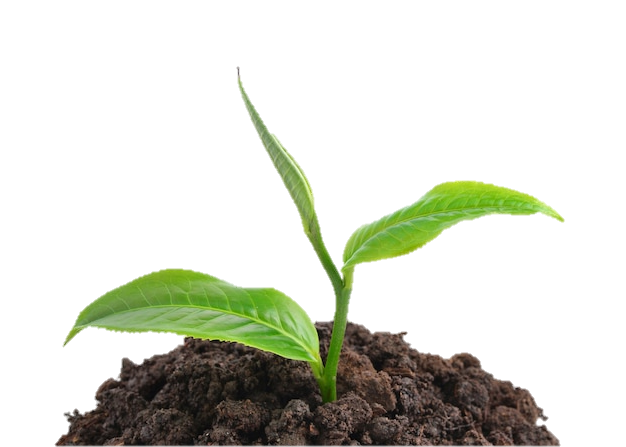
\includegraphics[width=0.4\textwidth]{images/Agro.png}
\end{frame}

\begin{frame}{Motivación del problema}
	\begin{block}{\centering Proceso de decisión}
		\begin{minipage}{0.5\textwidth}
			\begin{itemize}
				\item Conocimiento ancentral.
				\item Sistematización y mecanización.
				\item Estudios científicos.
				\item Interacciones multidisciplinarias.
			\end{itemize}
		\end{minipage}%
		\begin{minipage}{0.5\textwidth}
			\begin{itemize}
				\item Biotecnología y edición genética.
				\item Agricultura de precisión.
				\item Agricultura adaptativa.
				\item Modelación predictiva.
			\end{itemize}
		\end{minipage}
	\end{block}
	\centering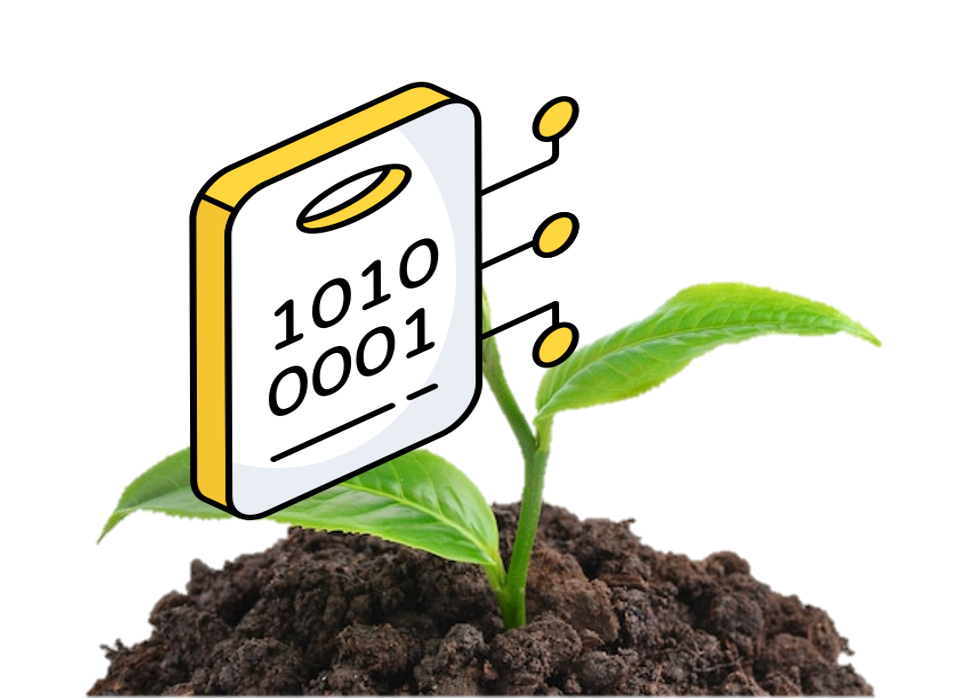
\includegraphics[width=0.4\textwidth]{images/Agrodatascience.png}
\end{frame}

\begin{frame}{Motivación del problemas}
	\begin{block}{\centering Trabajos previos}
		\begin{minipage}{0.5\textwidth}
			Cultivos anuales
			\begin{itemize}
				\item Hortalizas.
			\end{itemize}
		\end{minipage}%
		\begin{minipage}{0.5\textwidth}
			Cultivos perennes
			\begin{itemize}
				\item Árboles frutales.
			\end{itemize}
		\end{minipage}
	\end{block}
	\pause
	\centering\begin{minipage}{0.75\textwidth}
	\begin{block}{\bf Agave}
		\pause\,\,\,Anual\,\, --- Reproducción, trasplantación y {\bf producción}.\\
		\pause Perenne --- Inversión económica, rentabilidad y {\bf producción}. 
	\end{block}
\end{minipage}

\,\\

\pause\centering \Large  Simultáneamente, anual y perenne.
\end{frame}



\begin{frame}{Introducción: Cambio climático}
    \vspace{-1.5cm}
    \begin{block}{\centering Alteraciones a largo plazo en los patrones climáticos}
       \begin{minipage}{0.5\textwidth}
			\pause\begin{itemize}
				\item Aumento en las temperaturas.
                \item Aumento de incendios forestales.
			\end{itemize}
		\end{minipage}%
		\pause\begin{minipage}{0.5\textwidth}
			\begin{itemize}
				\item Disponibilidad de agua.
                \item Cambios en los suelos.
			\end{itemize}
		\end{minipage}
    \end{block}

    \begin{minipage}{0.5\textwidth}
			\pause\begin{block}{Factores naturales}
				\begin{itemize}
					\item Actividad solar.
					\item Erupciones volcánicas.
				\end{itemize}
			\end{block}
		\end{minipage}%
		\begin{minipage}{0.5\textwidth}
			\pause\vspace{0cm}\begin{block}{Factores humanos}
				\begin{itemize}
					\item Quema de combustibles fósiles.
					\item Actividad industrial. \phantom{p}
				\end{itemize}
			\end{block}
		\end{minipage}
        \,\\
    \hfill \scriptsize Fuente: ONU (2025).
\end{frame}

\begin{frame}{Introducción: Cambio climático}
\vspace{-1cm}

\begin{block}{\centering Consecuencias}
       \begin{minipage}{0.5\textwidth}
			\begin{itemize}
				\item Desplazamiento social.
                \item Reducción de la biodiversidad.
			\end{itemize}
		\end{minipage}%
		\begin{minipage}{0.5\textwidth}
			\begin{itemize}
				\item Problemas de salud.
                \item Alteraciones en la precipitación.
			\end{itemize}
		\end{minipage}
    \end{block}
    \pause
    \begin{block}{Desfase de las estaciones del año \hfill {\scriptsize Fuente: Wang \textit{et al.} (2021).}}
    \centering
        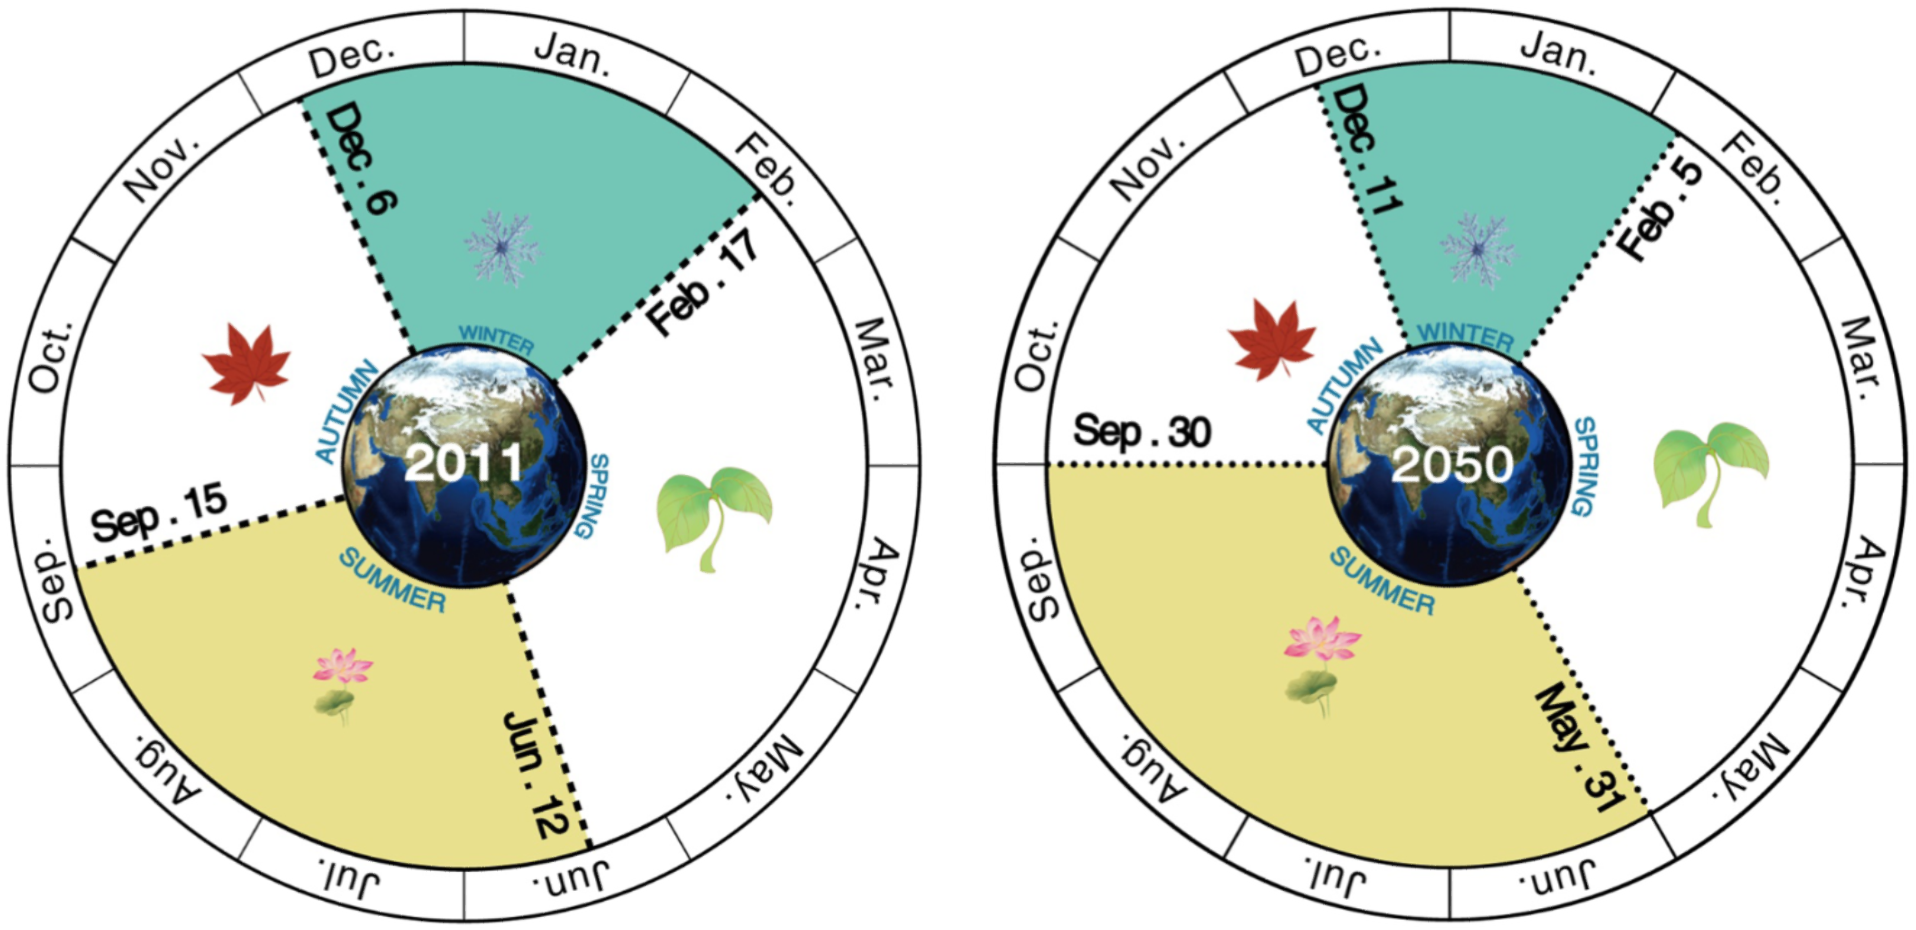
\includegraphics[scale=0.31]{images/Seasons.png}
    \end{block}
\end{frame}


\begin{frame}{Industria agrícola}
\vspace{-1cm}
\begin{minipage}{0.5\textwidth}
			\pause\begin{block}{Estabilidad}
			    \begin{itemize}
				\item Periodo luminoso.
                \item Temperaturas.
                \item Humedad.
                \item Características de suelo.
                \item Polinización.
                
			\end{itemize}
			\end{block}
		\end{minipage}%
		\begin{minipage}{0.5\textwidth}
		\pause\begin{block}{En ausencia}
			\begin{itemize}
                    \item Problemas de seguridad alimentaria.
                    \item Desequilibrio en la cadena trófica.
                    \pause
                    \item Desabasto en industrias dependientes.
                    \item Problemas económicos.
                    \item Conflictos sociales.
			\end{itemize}
			\end{block}
		\end{minipage}
\pause
        \centering
        \,\\ \Large
La agricultura es fundamental para un desarrollo integral.
\end{frame}


\begin{frame}{Aguacates}
    \vspace{-1cm}
    \begin{minipage}{0.5\textwidth}
			\hspace{-0.5cm}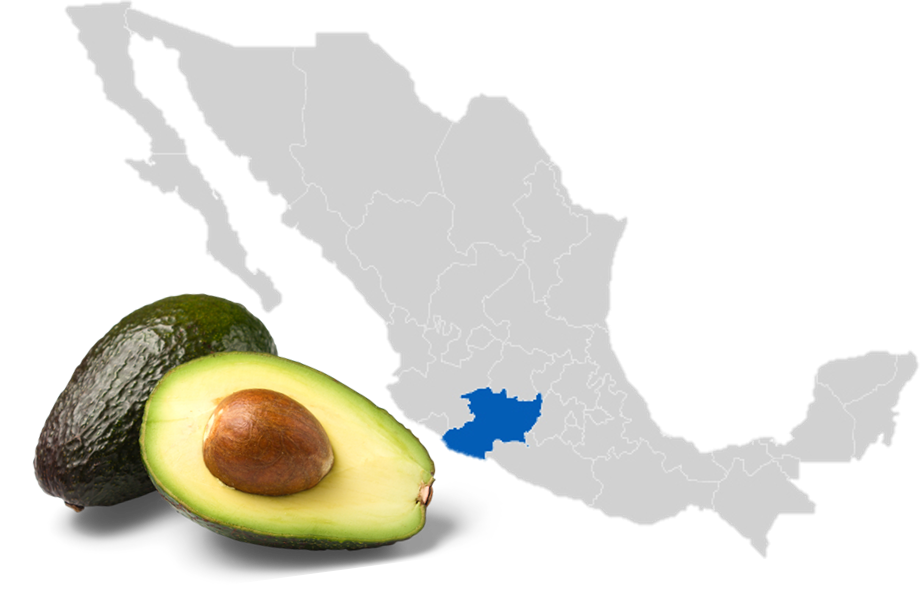
\includegraphics[width=\textwidth]{images/Location.png}
		\end{minipage}%
		\begin{minipage}{0.5\textwidth}
            \begin{block}{Fenología}
                \begin{itemize}
				\item Suelos con pH de 5.5 -- 7.
                    \item Precipitaciones anuales de 1200 mm. uniformemente distribuidas.
                    \item Ausencia de heladas.
                    \item Ausencia de vientos calurosos secos.
                    \item Altitudes de 800 -- 1200 m.s.n.m.
                    \item Temperaturas de 12$^\circ$ C -- 30$^\circ$ C. 
			\end{itemize}
            \end{block}
		\end{minipage}
        \,\\
        \hfill {\scriptsize Fuente: SAGARPA (2017); Salinas Vargas \textit{et al.} (2021).}
\end{frame}



\begin{frame}{Ciclo productivo del aguacate}
    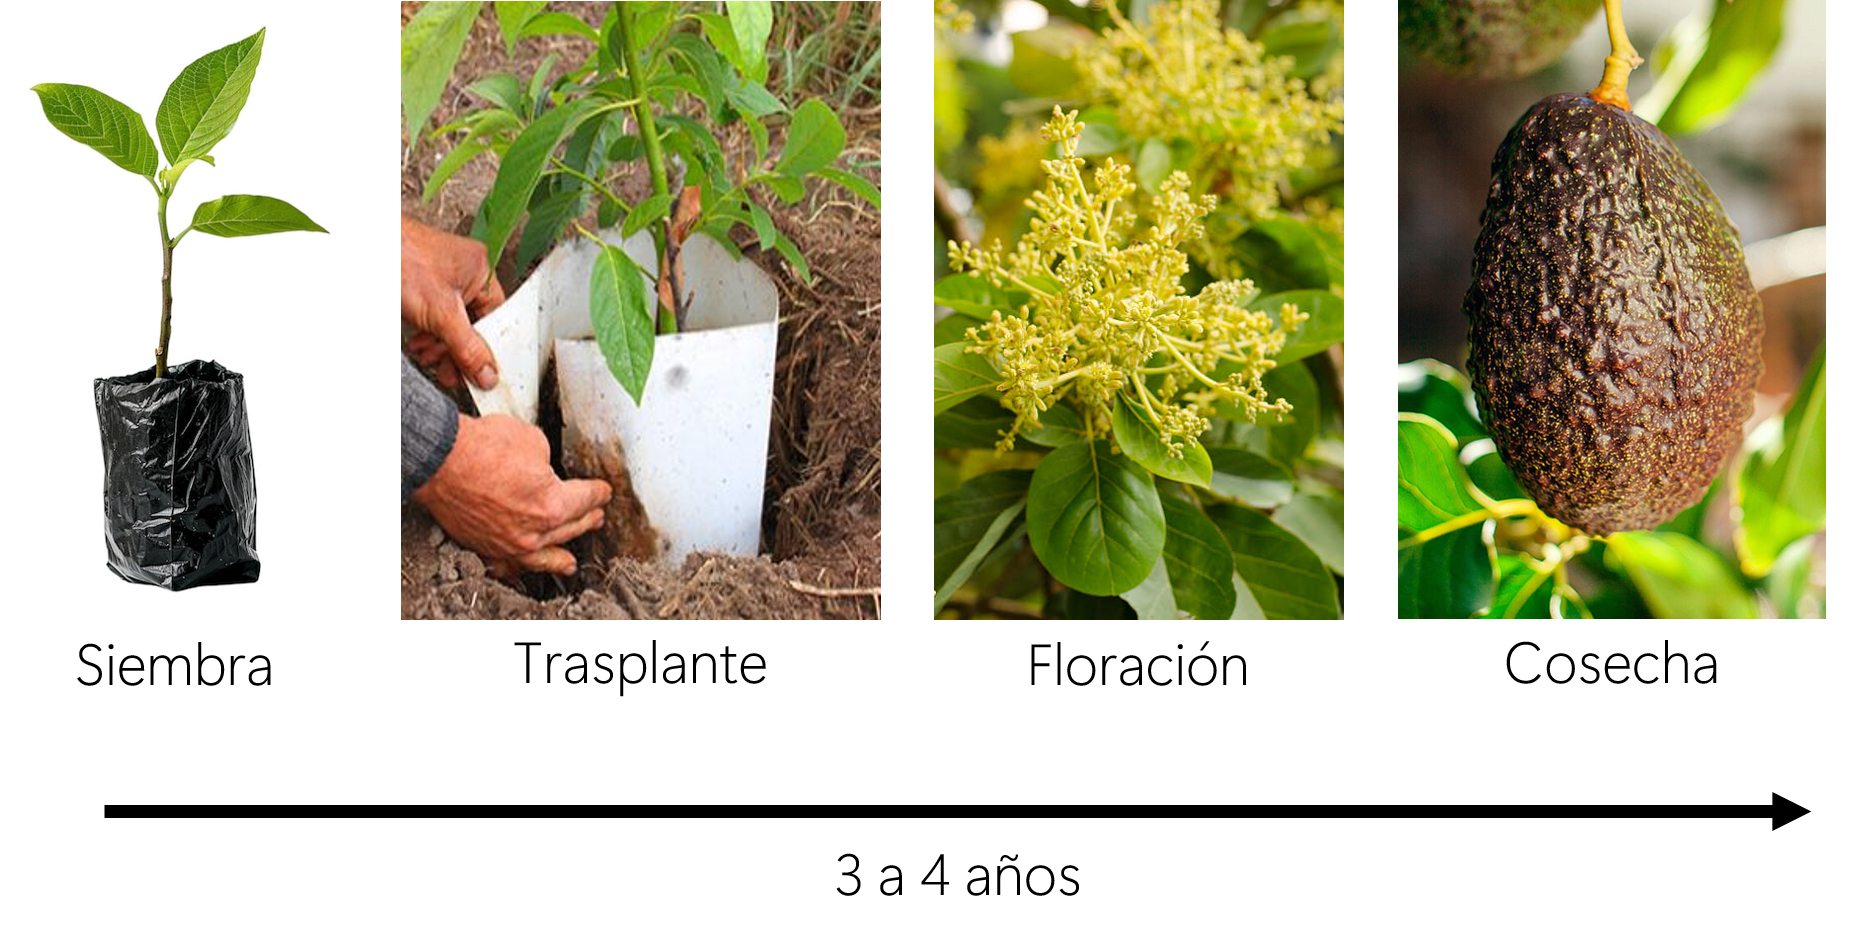
\includegraphics[width=\textwidth]{images/ProductiveCycle.png}
\end{frame}

\begin{frame}{Siembra}
    \vspace{-1cm}
		\begin{minipage}{0.5\textwidth}
            \begin{block}{}
                \begin{itemize}
				\item Se desarrolla en viveros.
                    \item Se realiza de marzo a mayo.
                    \item Duración de entre 10 -- 12 meses.
			\end{itemize}
            \end{block}
            \pause\,\\
            \begin{block}{Es una etapa muy controlada.}
            \end{block}
		\end{minipage}%
        \begin{minipage}{0.5\textwidth}
        \centering
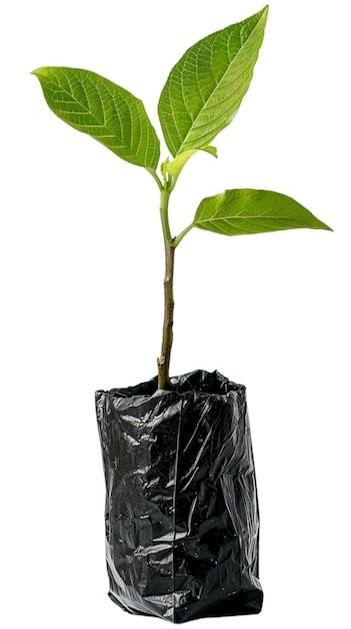
\includegraphics[height=0.7\textheight ]{images/Vivero.jpg}
		\end{minipage}%
        \,\\
        \hfill {\scriptsize Fuente: SAGARPA (2017); Campos–Rojas \textit{et al.} (2012).}
\end{frame}

\begin{frame}{Trasplante}
    \vspace{-1cm}
    \begin{minipage}{0.5\textwidth}
			\hspace{-0.5cm}
            \centering
            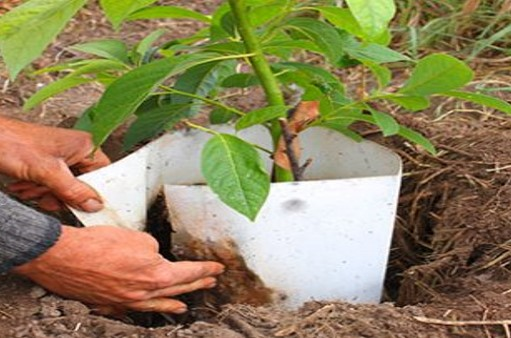
\includegraphics[height=0.7\textheight ]{images/Trasplante.jpg}
		\end{minipage}%
		\begin{minipage}{0.5\textwidth}
            \begin{block}{}
                \begin{itemize}
				\item Reubicación final al suelo.
                    \item En el verano, no es recomendable.
                    \item Existe un periodo crítico de cuatro semanas.
			\end{itemize}
            \end{block}
            \pause
            \begin{block}{Impacto del trasplante}
                \begin{itemize}
				\item Es un periodo de \textit{aclimatación}.
                    \item Estrés en la planta.
                    \item Pérdidas en el número de plantas.
			\end{itemize}
            \end{block}
		\end{minipage}
        
        \,\\
        \hfill {\scriptsize Fuente: SAGARPA (2017); Salinas Vargas \textit{et al.} (2021); Premkumar \textit{et al.} (2002).}
\end{frame}


\begin{frame}{Floración}
    \vspace{-1cm}
		\begin{minipage}{0.5\textwidth}
            \begin{block}{}
                \begin{itemize}
				\item Antesala de la producción.
                    \item El desarrollo floral sucede en el otoño e invierno.
                    \item Requiere de periodos nocturnos largos
                    \item Tres semanas con temperaturas bajas y una semana con una elevación en temperaturas. 
			\end{itemize}
            \end{block}
		\end{minipage}%
        \begin{minipage}{0.5\textwidth}
        \centering
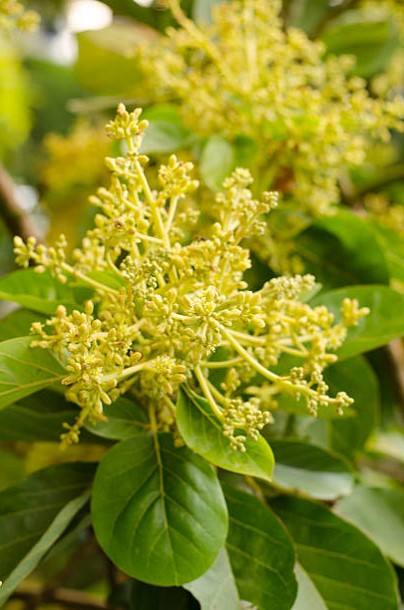
\includegraphics[height=0.7\textheight ]{images/Floración.jpg}
		\end{minipage}%
        \,\\
        \hfill {\scriptsize Fuente: Salinas Vargas \textit{et al.} (2021); Acosta-Rangel \textit{et al.} (2021).}
\end{frame}

\begin{frame}{Cosecha}
    \vspace{-1cm}
    \begin{minipage}{0.5\textwidth}
			\hspace{-0.5cm}
            \centering
            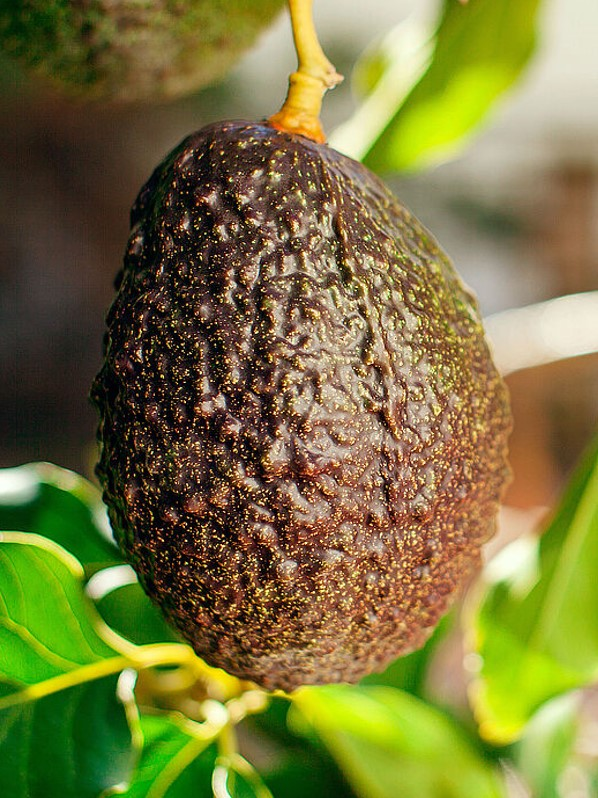
\includegraphics[height=0.7\textheight ]{images/Fruto.jpg}
		\end{minipage}%
		\begin{minipage}{0.5\textwidth}
            \begin{block}{}
                \begin{itemize}
                    \item En México, es un proceso continuo.
				\item La primera cosecha comercial se obtiene a los 3 o 4 años de edad.
                    \item Un árbol produce aproximadamente 75 Kg por año.  
                    \item La producción se estabiliza a los 8 años de edad.
                    \item La producción máxima es de 200 Kg por año.
                    \item Vida productiva de 40 años que decae a partir de los 30 años.
			\end{itemize}
            \end{block}
		\end{minipage}
        \,\\
        \hfill {\scriptsize Fuente: Peña-Urquiza \textit{et al.} (2015); Mosquera \textit{et al.} (2015).}
\end{frame}


\begin{frame}{Aguacates en Michoacán}
    \vspace{-1cm}
		\begin{minipage}{0.5\textwidth}
            \begin{block}{}
                \begin{itemize}
				\item Producción anual mayor a 2.2 millones de toneladas.
                    \item Genera el 77.43\% de la producción nacional.
                    \item El 60.18\% de sus municipios participan.
                    \item Destinan 187000 hectáreas para el cultivo.
			\end{itemize}
            \end{block}
		\end{minipage}%
        \begin{minipage}{0.5\textwidth}
\hspace{-0.5cm}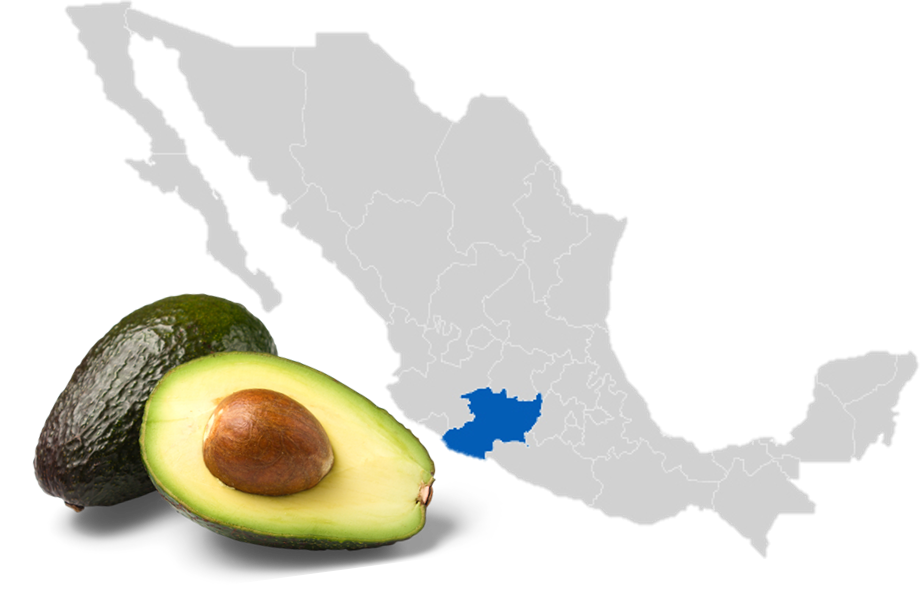
\includegraphics[width=\textwidth]{images/Location.png}
		\end{minipage}%
        \,\\
        \hfill {\scriptsize Fuente: SIAP (2025-1); SIAP (2025-2).}
\end{frame}


\section{¿Cómo pueden utilizarse técnicas de aprendizaje automático, considerando información agroclimática, para predecir la evolución del proceso productivo del aguacate seccionándolo en las distintas etapas que lo compone?}


\begin{frame}\frametitle<1>{\hfill Siembra}
\frametitle<2>{\hfill Siembra}
\frametitle<3>{\hfill Siembra}
\frametitle<4>{Trasplante}
    \vspace{-1cm}
		\begin{minipage}{0.5\textwidth}
            \vspace{-6cm}\begin{block}{}
                \begin{itemize}
				\item Considera el sistema de unidades de calor.
                    \item Se adapta a las condiciones de la planta.
                    \item Algoritmos de decisión simple.
                    \item Determinan periodos en los cuales las condiciones climáticas favorecen la viabilidad de la semilla sembrada.
			\end{itemize}
            \end{block}
		\end{minipage}%
        \begin{minipage}{0.5\textwidth}
        \vspace{0.5cm}
        
        \begin{overprint}
\onslide<1>\centering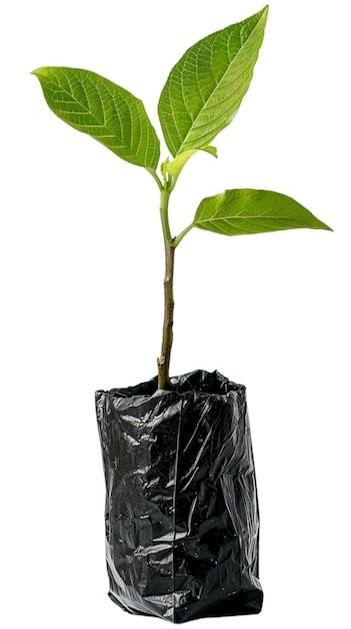
\includegraphics[height=0.7\textheight]{images/Vivero.jpg}\\\hfill {\scriptsize Fuente: Elnesr \textit{et al.} (2013); Elnesr \textit{et al.} (2016); Callejas-Rodríguez \textit{et al.} (2023).}
\onslide<2>  \centering\vspace{1cm}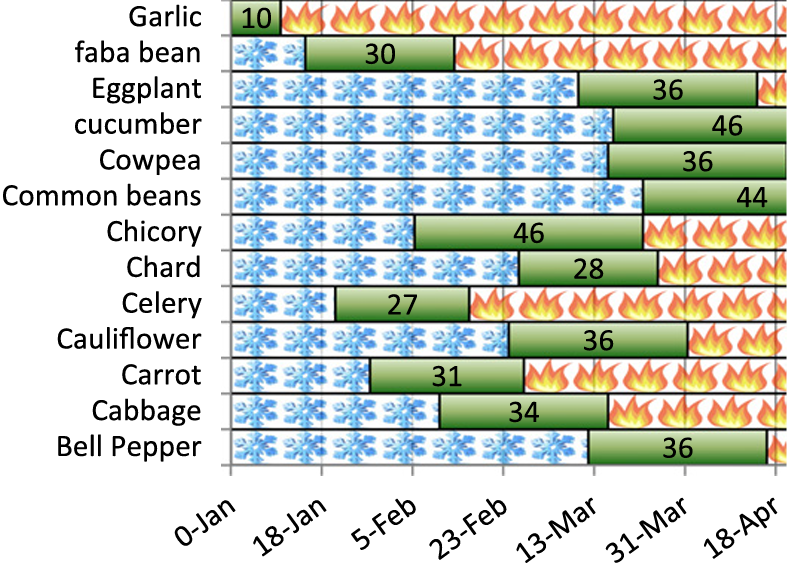
\includegraphics[height=0.5\textheight]{images/Elnesr.png}\\\hfill {\scriptsize Fuente: Elnesr \textit{et al.} (2013); Elnesr \textit{et al.} (2016); Callejas-Rodríguez \textit{et al.} (2023).}
\onslide<3>  \centering\vspace{1cm}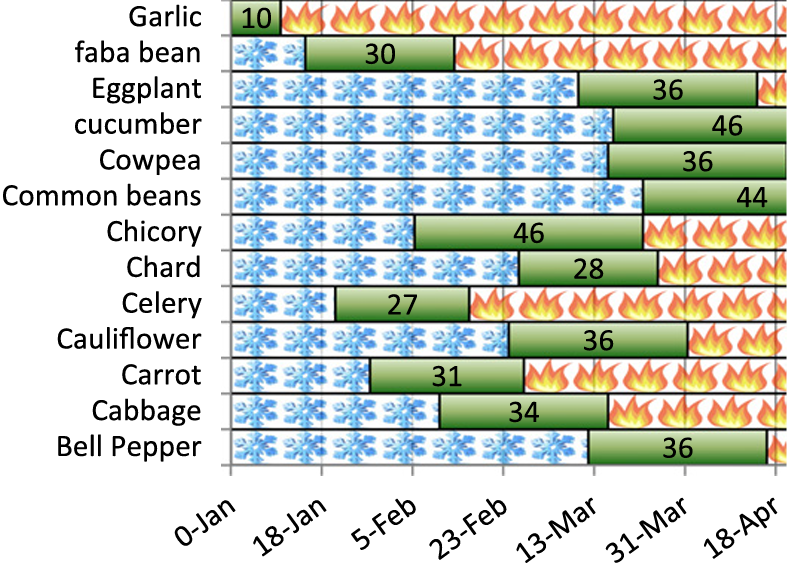
\includegraphics[height=0.5\textheight]{images/Elnesr.png}\\\hfill {\scriptsize Fuente: Elnesr \textit{et al.} (2013); Elnesr \textit{et al.} (2016); Callejas-Rodríguez \textit{et al.} (2023).}
\onslide<4>  \centering\vspace{1cm}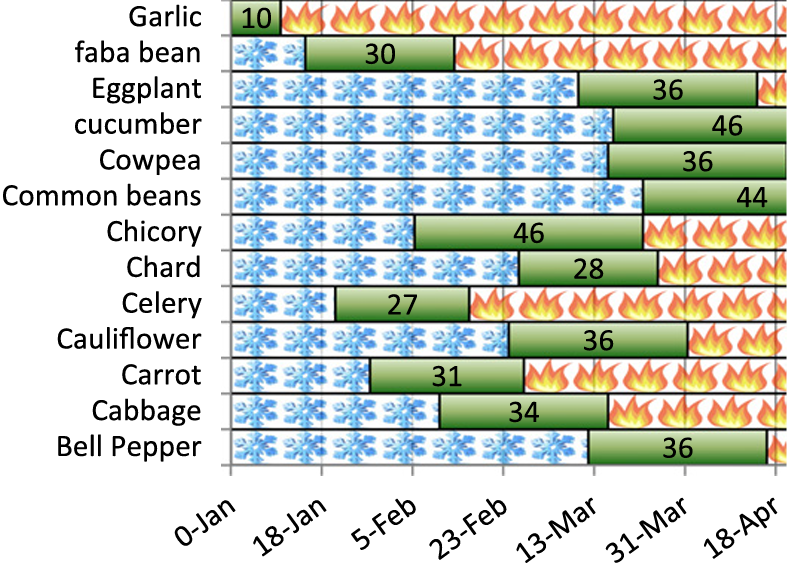
\includegraphics[height=0.5\textheight]{images/Elnesr.png}\\\hfill {\scriptsize Fuente: Elnesr \textit{et al.} (2013); Elnesr \textit{et al.} (2016); Callejas-Rodríguez \textit{et al.} (2023).}
        \end{overprint}
		\end{minipage}
        \pause
        \begin{minipage}{0.5\textwidth}
            \pause\vspace{-12.5cm}\begin{block}{\centering Etapa muy controlada}
            \end{block}
        \end{minipage}
\end{frame}


\begin{frame}{Floración}
    \vspace{0cm}
    \begin{minipage}{0.5\textwidth}
	   \vspace{-0.8cm}
            \centering
            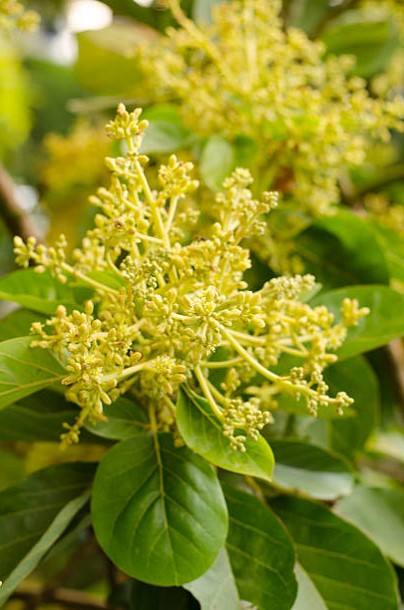
\includegraphics[width=0.7\textwidth]{images/Floración.jpg}
		\end{minipage}%
		\begin{minipage}{0.5\textwidth}
            \vspace{-1cm}\begin{block}{}
                \begin{itemize}
				\item Emplea el concepto de días frío acumulado (DFA).
                \item Temperatura del aire.
                    \item Base de datos con registros de 2 años.
                    \item Estudia la formación de yemas.
                    \item Emplea regresiones polinomiales (grado 6).
                    \end{itemize}
            \end{block}
		\end{minipage}\\
    %\vspace{-1cm}
    \hfill {\scriptsize Fuente:Salazar-García \textit{et al.} (2018).}
\end{frame}

\begin{frame}{Producción}
    
    \vspace{-1cm}
		\begin{minipage}{0.5\textwidth}
            \begin{block}{}
                \begin{itemize}
				\item Registros de Turquía desde 1980 a 2015.
                    \item La serie de tiempo es no estacionaria, con tendencia y sin estacionalidad.
                    \item Aplica los modelos de suavizamiento exponencial de Holt, Damped y Brown.
                    \item Genera un pronóstico para el periodo 2016-2025. 
			\end{itemize}
            \end{block}
		\end{minipage}%
        \begin{minipage}{0.5\textwidth}
        \centering
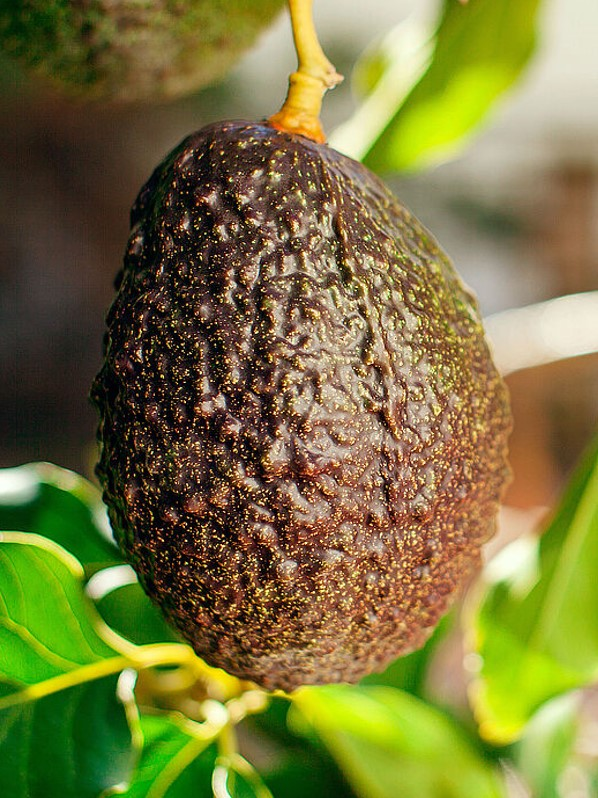
\includegraphics[height=0.7\textheight ]{images/Fruto.jpg}
		\end{minipage}%
        \,\\
        \hfill {\scriptsize Fuente: Akin \textit{et al.} (2017).}
\end{frame}

\begin{frame}{Producción}
    \vspace{-1cm}
    \begin{minipage}{0.5\textwidth}
			\hspace{-0.5cm}
            \centering
            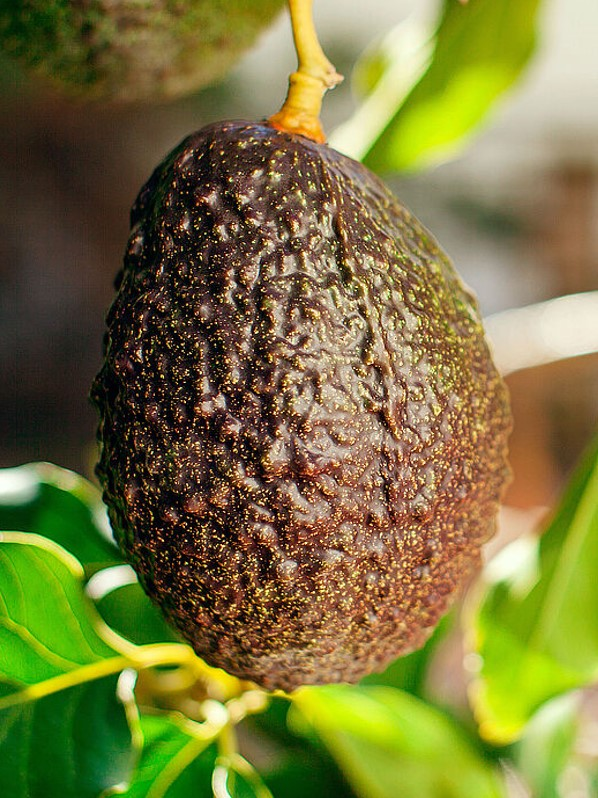
\includegraphics[height=0.7\textheight ]{images/Fruto.jpg}
		\end{minipage}%
		\begin{minipage}{0.5\textwidth}
            \begin{block}{}
                \begin{itemize}
                    \item Instala sensores en una huerta de Huitzilac, Morelos.
				\item Registró temperaturas (suelo y ambiente), humedad, lúmenes y nutrientes.
                    \item Emplea algoritmos supervisados y no supervisados. 
                    \item Propone al algoritmo Random Forest Regressor como mejor estimador.
			\end{itemize}
            \end{block}
		\end{minipage}
        \,\\
        \hfill {\scriptsize Fuente: Arizmendi-Peralta (2024).}
\end{frame}

\begin{frame}{Producción}
    
    \vspace{-1cm}
		\begin{minipage}{0.5\textwidth}
            \begin{block}{}
                \begin{itemize}
				\item Compara la producción de árboles sanos respeto a enfermos.
                    \item Estima la producción por huerta con árboles de la misma edad.
                    \item Propone un modelo de regresión cuadrática. 
			\end{itemize}
            \end{block}
		\end{minipage}%
        \begin{minipage}{0.5\textwidth}
        \centering
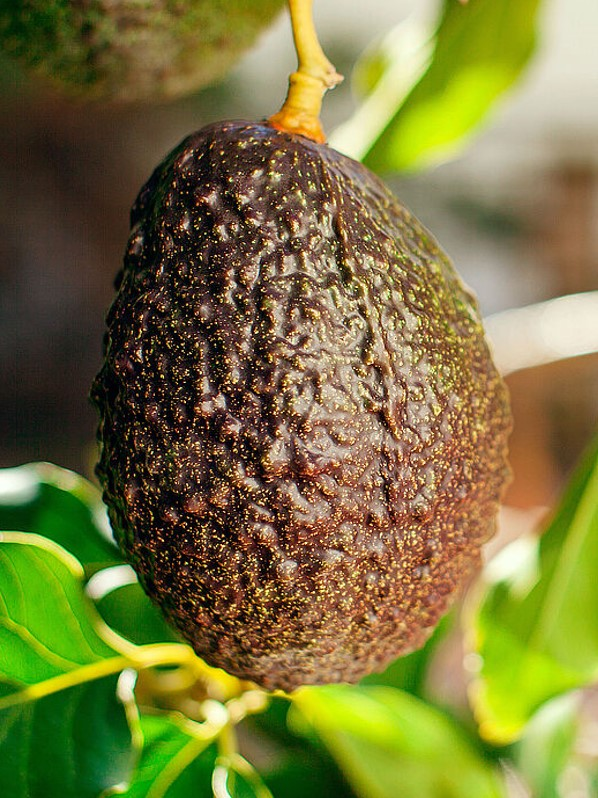
\includegraphics[height=0.7\textheight ]{images/Fruto.jpg}
		\end{minipage}%
        \,\\
        \hfill {\scriptsize Fuente: Mosquera \textit{et al.} (2015).}
\end{frame}

\begin{frame}{Objetivos generales}
    Proponer un modelo de predicción, basado en aprendizaje automático, para pronosticar

    \begin{minipage}{0.33\textwidth}
        \pause\begin{block}{Trasplante}
            Periodos ideales.
        \end{block}
    \end{minipage}%
    \begin{minipage}{0.34\textwidth}\pause\begin{block}{Floración \phantom{p}}
            Producción de flores.
        \end{block}%
    \end{minipage}%
    \begin{minipage}{0.33\textwidth}
        \pause\begin{block}{Cosecha \phantom{p}}
            Producción de frutos.
        \end{block}
    \end{minipage}
    
\,\\
   \pause
   Empleando datos agroclimáticos disponibles para el estado de Michoacán y contribuir en el fortalecimiento del proceso productivo del aguacate.
\end{frame}

\begin{frame}{Datos disponibles}
    \vspace{-1cm}
    \begin{minipage}{0.5\textwidth}
			\hspace{-0.5cm}
            \centering
            
\includegraphics[width=\textwidth]{images/Essenger.png}
		\end{minipage}%
		\begin{minipage}{0.5\textwidth}
            \begin{block}{}
                \begin{itemize}
                    \item Instituto Nacional de Investigaciones Forestales, Agrícolas y Pecuarias.
				\item Registros diarios de estaciones climáticas.
                    \item Periodo de enero de 1980 a diciembre de 2022.
                    \item Temperatura del aire.
                    \item Periodo luminoso.
                    \item Radiación de onda corta.
                    \item Lluvia líquida.
                    \item Presión de vapor.
			\end{itemize}
            \end{block}
		\end{minipage}
\end{frame}
\begin{frame}{Datos disponibles}
    \vspace{-1cm}
		\begin{minipage}{0.5\textwidth}
            \begin{block}{}
                \begin{itemize}
                    \item INIFAP.
				\item Datos medidos en diversas profundidades.
                    \item Rango de 0 a 200 cm.
                    \item Porción de limo.
                    \item Capacidad de intercambio catiónico.
                    \item Nitrógeno.
                    \item Carbono orgánico.
                    \item pH.
			\end{itemize}
            \end{block}
		\end{minipage}%
        \begin{minipage}{0.5\textwidth}
			\hspace{0cm}
            \centering
            
\includegraphics[width=\textwidth]{images/MSMx.png}
		\end{minipage}
\end{frame}

\begin{frame}{Datos disponibles}
    \vspace{-1cm}
    \begin{minipage}{0.5\textwidth}
			\hspace{-0.5cm}
            \centering
            
\includegraphics[width=\textwidth]{images/conagua.png}
		\end{minipage}%
		\begin{minipage}{0.5\textwidth}
            \begin{block}{}
                \begin{itemize}
                    \item Sistema Meteorológico Nacional.
				\item Registros diarios a nivel estatal.
                    \item Periodo de enero de 1960 a abril de 2025.
                    \item Temperatura ambiental.
                    \item Evaporación.
                    \item Precipitación.
                    \item Lluvia líquida.
			\end{itemize}
            \end{block}
		\end{minipage}
\end{frame}

\begin{frame}{Datos disponibles}
    \vspace{-1cm}
		\begin{minipage}{0.5\textwidth}
            \begin{block}{}
                \begin{itemize}
                    \item Servicio de Información Agroalimentaria y Pesquera.
				\item Avance y cierre de siembras y cosechas desde 2018 a la fecha.
                    \item Reportes mensuales a nivel municipal y estatal.
                    \item Hectáreas sembradas.
                    \item Hectáreas cosechadas.
                    \item Hectáreas siniestradas.
                    \item Producción (ton).
                    \item Rendimiento (ton/Ha).
			\end{itemize}
            \end{block}
		\end{minipage}%
        \begin{minipage}{0.5\textwidth}
			\hspace{0cm}
            \centering
            
\includegraphics[width=\textwidth]{images/siap.png}
		\end{minipage}
\end{frame}



\begin{frame}{Conclusión}
    \vspace{-1cm}\begin{minipage}{0.7\textwidth}
        \begin{block}{Métodos}
            \begin{itemize}
                \item Algoritmos de decisión simple.
                \item Modelos de suavizamiento exponencial.
                \item Regresiones.
                \item Perceptrón multicapa.
                \item Support vector machine.
                \item Árboles de decisión.
                \item Bosques aleatorios.
                \item M5 Prime.
            \end{itemize}
        \end{block}
    \end{minipage}%
    \begin{minipage}{0.3\textwidth}
        \pause\begin{block}{Ubicaciones}
            \begin{itemize}
                \item Turquía.
                \item Morelos.
                \item Jalisco.
            \end{itemize}
        \end{block}
    \end{minipage}
\end{frame}


\begin{frame}{Preliminares}

\vspace{-1cm}\begin{block}{}
    Se han estudiado los municipios de Los Reyes y Tacámbaro, Michoacán.\\

\,\\

    \begin{minipage}{0.5\textwidth}
        \begin{itemize}
        \item Periodo luminoso.
        \item Radiación de onda corta.
        \item Temperatura (máxima y mínima) del aire.
    \end{itemize}
    \end{minipage}%
    \begin{minipage}{0.5\textwidth}
        \begin{itemize}
        \item Precipitación diaria
        \item Presión media de evaporación del agua.
    \end{itemize}
    \end{minipage}%
\end{block}

Encontrando correlaciones positivas y negativas, estadísticamente significativas, respecto a la producción y rendimiento.
\end{frame}

\section*{Referencias}
\begin{frame}[allowframebreaks,noframenumbering]{Referencias}
	\vspace*{-1cm}
	\tiny
	\bibliography{Bibliografia.bib}
	\bibliographystyle{alpha}
	\nocite{*}
	%\printbibliography
\end{frame}

\section*{Gracias}
\begin{frame}[noframenumbering]
%\vspace{2cm}
     \begin{center}
	    \Huge{Gracias}
	\end{center}
    \end{frame}
\end{document}